\documentclass[12pt]{article}
\author{Giulio Incoronato, Antonio Mazzarella}
\usepackage{graphicx}
\usepackage{fancyhdr}
\usepackage{hyperref}
\usepackage{lipsum} %for some dummy text
\usepackage{array} %per gli array in tabella
\usepackage[table]{xcolor} %colori della tabella
\newcommand{\mytextbf}[1]{\textbf{\bfseries #1}}
\usepackage{tabularx}
\usepackage{geometry}
\usepackage{pgf-pie}
\usepackage[T1]{fontenc}


%variabili globali
\newcommand{\mainname}{UGotTheJob}


\geometry{
    a4paper,
    total={170mm,257mm},
    left=20mm,
    top=20mm,
}


%di seguito imposterò i piè pagina
\pagestyle{fancy}
\fancyhf{}
\fancyfoot[L]{\thepage}
\fancyfoot[R]{
\includegraphics[height=40pt]{job_seeking.png}}
\setlength{\footskip}{43.60004pt}

%font utilizzato san serif
\renewcommand{\headrulewidth}{0pt} % rimuovi la linea dell'header
\renewcommand{\familydefault}{\sfdefault}

\begin{document}
\thispagestyle{empty}

\begin{center}%inizio documento
    
\includegraphics[scale=0.6]{job_seeking.png}

    \vspace{1cm}

    \textbf{\huge{\mainname}} % Aggiunge il titolo

    \vspace{0.5cm}

    \fontsize{17}{16}
    \textbf{Artificial Intelligence DOCUMENT}

    \textit{"Dipartimento di Informatica anno 2022/2023"}

    \textit{"Professore: Fabio Palomba"}

    \vspace{1.8cm}


    \begin{table}[ht]
        \fontsize{17}{12}\selectfont
        \centering
        \setlength{\arrayrulewidth}{2pt}
        \setlength{\tabcolsep}{5pt}
        \def\arraystretch{1.8}
        \begin{tabular}{ c | c }
            \textbf{Autori}    & \textbf{Matricola} \\
            \hline
            Giulio Incoronato  & 0512111363         \\
            Antonio Mazzarella & 0512112830         \\
        \end{tabular}
    \end{table}
\end{center}

\newpage %nuova pagina

\tableofcontents

\newpage

\section{Introduzione}
Quante volte hai avuto l'ansia di essere preso o pure no in uno specifico lavoro?
Quante volte ti sei domandato se fossi giusto tu per quel lavoro? Con la fine del proprio percorso
di studio ci si pongono tante domande e dubbi se si viene presi in un determinato lavoro oppure no.
\par
Tutto questo sorge perchè dopo diversi anni di studio si vuole avere la sicurezza di essere presi
per il lavoro dei propri sogni. Sarebbe utile avere un tool in grado di
prevedere, attraverso dei dati, quantà probabilità hai di avere il lavoro.
\par
Il nostro team mira a combattere tutte queste ansie creando un tool chiamato \textbf{"\mainname"}
che integrerà un modello di machine learning supervisionato che andrà a prevedere la possibilità di essere piazzato.

\subsection{Link Utili}
\begin{enumerate}
    \item Questo è il link alla repository ufficiale di \textbf{\mainname}: \href{https://github.com/ShackWove/GuessUJob}{Link}
    \item Questo è il link dove abbiamo preso i dataset: \href{https://www.kaggle.com/datasets/ahsan81/job-placement-dataset}{Link}
    \item Qui è dove è stata presa l'icona del nostro tool: \href{https://www.flaticon.com/free-icon/job-seeking_1503438}{Link}
\end{enumerate}

\section{Specifiche P.E.A.S.}

\begin{table}[ht]
    \centering
    \rowcolors{1}{gray!5}{gray!15}
    \begin{tabular}{| l | m{8cm} |}
        \hline
        \textbf{Performance} & Capacità dell'agente di prevedere se l'utente sarà preso o meno per un lavoro.                       \\
        \textbf{Enviroment}  & L'ambiente in cui l'agente opera rappresentato da un form di cui l'utente scriverà i dati necessari. \\
        \textbf{Actuators}   & Interfaccia utente dell'applicazione dove uscirà il valore predetto.                                 \\
        \textbf{Sensors}     & Form nell'interfaccia utente.                                                                        \\
        \hline
    \end{tabular}
    \caption{Tabella PEAS}
\end{table}
\subsection{Proprietà dell'Ambiente}
L'ambiente possiede le seguenti proprietà:
\begin{itemize}
    \item \textbf{Completamente osservabile:} l'agente ha accesso completo a tutte le informazioni fornite dall'utente.
    \item \textbf{Deterministico:} lo stato dell'ambiente dipende dall'azione intrapresa dall'agente.
    \item \textbf{Sequenziale:} le decisioni dell'agente dipendono dagli input dell'utente.
    \item \textbf{Statico:} nel momento in cui l'agente sta elaborando la sua previsione l'utente non può modificare il form dato in partenza.
    \item \textbf{Discreto:} le previsioni dell'agente dipendono soprattutto dagli input inseriti dall'utente, oltretutto c'è un numero limitato e preciso di informazioni che l'utente può inserire.
    \item \textbf{Singolo-agente:} esiste solo un agente che opera nell'ambiente.
\end{itemize}

\newpage

\section{Machine Learning}
Il machine learning (apprendimento automatico) è una tecnologia dell'intelligenza artificiale che consente alle macchine di imparare dai dati, senza essere esplicitamente programmate. In altre parole, il machine learning si basa sulla costruzione di algoritmi che possono imparare da un insieme di dati e migliorare la loro capacità di risolvere compiti specifici con l'esperienza.

Ci sono tre tipi principali di apprendimento automatico:
\begin{itemize}
    \item \textbf{Apprendimento supervisionato:} in questo tipo di apprendimento, il modello è addestrato su un insieme di dati che includono sia le caratteristiche di input che le relative etichette di output. Il modello usa queste etichette per adattarsi ai dati di input e fare previsioni su dati simili.
    \item \textbf{Apprendimento non supervisionato:} in questo tipo di apprendimento, il modello è addestrato su un insieme di dati senza etichette di output. Il modello cerca di scoprire pattern o strutture nei dati di input.
    \item \textbf{Apprendimento per rinforzo:} in questo tipo di apprendimento, il modello impara attraverso l'interazione con un ambiente dinamico. Il modello prende decisioni in base allo stato attuale dell'ambiente e riceve feedback sulle sue azioni.
\end{itemize}

Il machine learning viene utilizzato in molte applicazioni, tra cui la classificazione di immagini, la traduzione automatica, la diagnosi medica, la rilevazione di frodi e molto altro ancora.
Per il nostro tool abbiamo utilizzato un algoritmo di machine learning ad apprendimento supervisionato perché andremo a risolvere un problema di \textbf{classificazione}.

\section{CRISP-DM}
Per progettare una soluzione basata su machine learning bisogna avere un approccio \textbf{data and software engeneering}.
Per la creazione di tale software abbiamo utilizzato il modello \textit{CRISP-DM} (CRISP-DM è l’acronimo di Cross-Industry Standard Process for Data Mining.),
che rappresenta il ciclo di vita di progetti basati su intelligenza artificiale e data science.

Possiamo paragonare il modello \textit{CRISP-DM} ad un modello a cascata con feedback utilizzato per lo sviluppo di sistemi software
tradizionali. Presenta anche un modello \textbf{non sequenziale} in cui le diverse fasi possono essere eseguite un numero illimitato
di volte. Esistono diverse fasi raffigurate nell'immagine di seguito (Immagine 1):

\begin{center}
    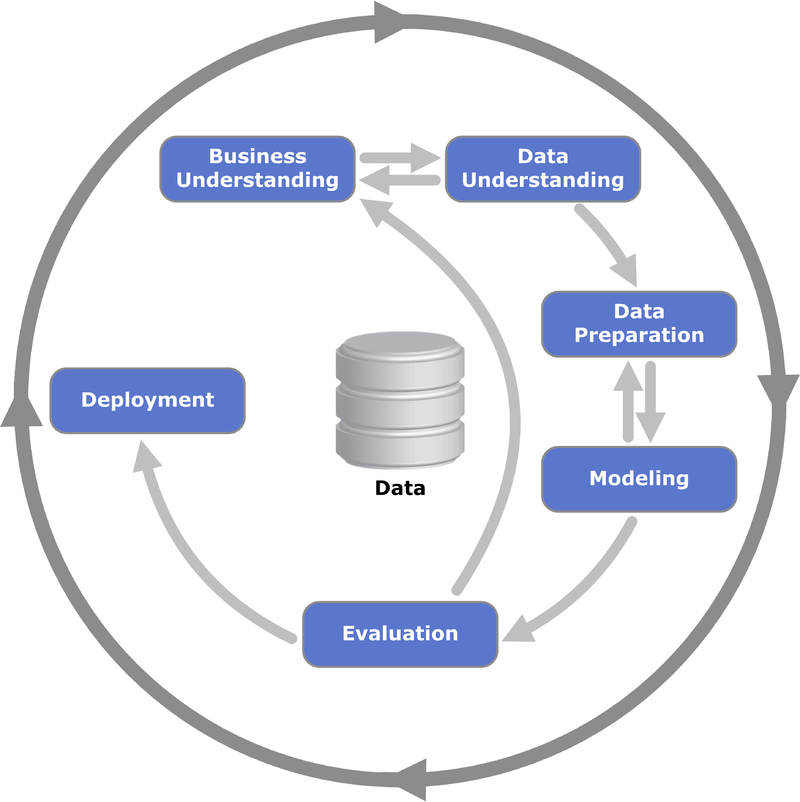
\includegraphics[scale=2.1]{CRISP-DM.png}

    \textit{Immagine 1}
\end{center}

\newpage

\subsection{Business Understanding}
In questa fase si raccolgono e definiscono gli obiettivi di Business che si vogliono raggiungere, oltre a determinare
la disponibilità delle risorse, stimare i rischi, indicare tecnologie e gli strumenti utilizzati per raggiungere gli obiettibi
prefissati.

\begin{itemize}
    \item \textbf{Obiettivi di Business:} L'obiettivo principale di \textbf{\mainname} è la realizzazione di un tool con cui l'utente interagisce inserendo
          dei dati richiesti in partenza sul suo percorso di studi, il tutto verrà analizzato e processato per poi dare in
          output la probabilità di essere piazzati o non.

    \item \textbf{Disponibilità delle risorse:} La risorsa che utilizzeremo per il nostro software sarà un dataset che conterrà
          le informazioni sui collocamenti in base ai vari percorsi di studio e esperienze pregresse. Per reperire questo dataset utilizzeremo una piattaforma importante che è \href{https://www.kaggle.com/}{Kaggle}.

    \item \textbf{Stima dei rischi:} I rischi che incontreremo saranno di tipo perlopiù Etico/Morale in quanto il dataset non fornisce una bilanciata percentuale di dati ad esempio tra persone di
          sesso differente.

    \item \textbf{Tecnologie e Strumenti:} Per analizzare, acquisire e modellare il dataset utilizzeremo il linguaggio \textit{Python} che presenta alcune librerie come \textbf{Pandas}, \textbf{sklearn}, \textbf{seaborn} ed etc.

\end{itemize}

\subsection{Data Understanding}
Come già discusso nella \textit{Stima dei rischi (parag. 4.1 Business Understanding)} il problema da noi riscontrato è stata la poca imparzialità che l'agente potesse avere
con il dataset da noi utilizzato. Il dataset avendo un discreto bilanciamento dei dati relativi al gender \textit{(vedi Figure 1)}, avrebbe portato al nostro agente una poco
corretta previsione del piazzamento di una persona, rischiando quindi di cadere in una discriminazione di tipo Etico/Morale di gender.
\begin{figure}[ht]
    \centering
    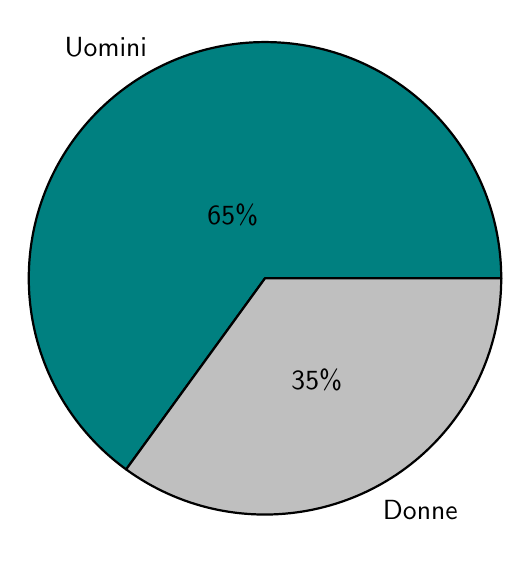
\begin{tikzpicture}
        \pie[color={teal, lightgray}]{65/Uomini, 35/Donne}
    \end{tikzpicture}
    \caption{Gender Dataset}
    \label{fig:torta}
\end{figure}

Il dataset inoltre presenta dati, come voti o specializzazioni, che non sono inerenti all'ambiente italiano. Possiamo vedere una lista con le descrizioni delle singole feature presenti:

%tabella descrizione feature

\begin{itemize}
    \item \textbf{Gender}: Indica appunto il \textit{sesso} della persona (M o F).
    \item \textbf{SSC Percentage}: Si riferisce generalmente all'esame di fine anno in India o in altri paesi. Indica una percentuale di voti ottenuti dallo studente in quel determinato esame. Sarebbe l'equivalente di un esame di \textbf{scuola media}.
    \item \textbf{HSC Percentage}: Si riferisce generalmente all'esame di fine anno in India o in altri paesi. Indica una percentuale di voti ottenuti dallo studente in quel determinato esame. Sarebbe l'equivalente di un esame di \textbf{scuola superiore}.
    \item \textbf{SSC Board}: Si riferisce generalmente al consiglio o all'ente che organizza l'esame di fine anno delle \textbf{scuole medie} in India. \par Col valore \textit{Central} si riferisce al CBSE (Central Board of Secondary Education), che sarebbe un organismo nazionale che organizza esami standardizzati per scuole pubbliche e private in India. \par Con Other si riferisce a consigli Statali o regionali.
    \item \textbf{HSC Board}: Si riferisce generalmente al consiglio o all'ente che organizza l'esame di fine anno delle \textbf{scuole superiori} in India. \par Col valore \textit{Central} si riferisce al CBSE (Central Board of Secondary Education), che sarebbe un organismo nazionale che organizza esami standardizzati per scuole pubbliche e private in India. \par Con Other si riferisce a consigli Statali o regionali.
    \item \textbf{HSC Subject}: Si riferisce alle materie che gli studenti devono studiare e superare per completare l'esame di fine anno dell'ultimo anno di \textbf{scuole superiori}. \par Questa variabile presenta tre tipi: \textit{Commerce, Science e Arts}.
    \item \textbf{Degree Percentage}: Indica la percentuale di punteggio ottenuta dagli studenti in un programma di Laurea.
    \item \textbf{Undergrad Degree}: È un titolo di studio che gli studenti ottengono dopo aver completato un programma di studi Universitari. \par Ci sono tre valori: \textit{Sci\&Tech, Comm\&Mgmt e Others}.
    \item \textbf{Work Experience}: Questa variabile, banalmente, rappresenta se il sottoscritto ha avuto o meno esperienza lavorativa pregressa.
    \item \textbf{Employee Test \%}: Rappresenta la percentuale del test di idoneità per una posizione di lavoro effettuato presso l'azienda in cui il candidato ha fatto domanda.
    \item \textbf{Specialization}: Rappresenta di che tipo di Specializzazione il candidato è in possesso. \par Questo dataset presenta 2 opzioni: \textit{Mkt\&Fin e Mkt\&HR}. Rispettivamente sono \textit{Mercato e Finanza} e \textit{Mercato e Risorse Umane} (Human Resource).
    \item \textbf{MBA Percentage}: Indica la percentuale di punteggio calcolata come media di voti di tutto il percorso di studi post-Laurea che si concentra sull'Amministrazione aziendale e sulla Gestione.
    \item \textbf{Status}: Indica, banalmente, se il candidato è piazzato o meno.
\end{itemize}

Questo ci porta a lavorare per un modello che non potrà essere utilizzato in una realtà italiana.

\newpage

\subsection{Data Preparation}
In questa sezione, tratteremo le tecniche adottate per preparare i dati acquisiti in modo che il nostro machine learner
non darà problemi e sarà quanto più efficiente possibile.

Il data preparation si articola nei seguenti quattro passaggi:

\begin{enumerate}
    \item \textbf{Data cleaning;}
    \item \textbf{Feature scaling;}
    \item \textbf{Feature selection;}
    \item \textbf{Data balancing;}
\end{enumerate}

\subsubsection{Data cleaning}
Il \textit{Data Cleaning}, definito come \textit{"Pulizia dei dati"}, si occupa di rimediare a problemi quando ci sono righe
di dati mancanti ma più in generale ha come obiettivo quello di fornire un dataset dotato di una qualità adeguata.
Nel nostro dataset non sono presenti dati mancanti e di conseguenza non abbiamo effettuato la fase di \textit{Data Imputation}.

\subsubsection{Feature scaling}
Il \textit{Feature Scaling} è l'insieme di tecniche che consentono di normalizzare o scalare un insieme di valori di una caratteristica.
Questa tecnica viene eseguita quando abbiamo dei valori estremamente diversi di una determinata caratteristica rispetto ad un altra.
Nel nostro caso non abbiamo avuto bisogno di normalizzare o scalare i valori del nostro dataset, in quanto non sono particolarmente diversi tra di loro.


\subsubsection{Feature selection}
La \textit{Feature selection} rientra nell'ambito del feature engeneering, che sarebbe il processo nel quale il progettista
utilizza la propria conoscenza del dominio per determinare le caratteristiche (feature) dai dati grezzi estraibile tramite tecniche
di data mining.

Nel nostro caso abbiamo pensato di rimuovere colonne che non erano adeguate per il nostro obiettivo ovvero, quello di creare
un software che preveda un piazzamento nel mondo del lavoro quanto più etico possibile.

\begin{center}
    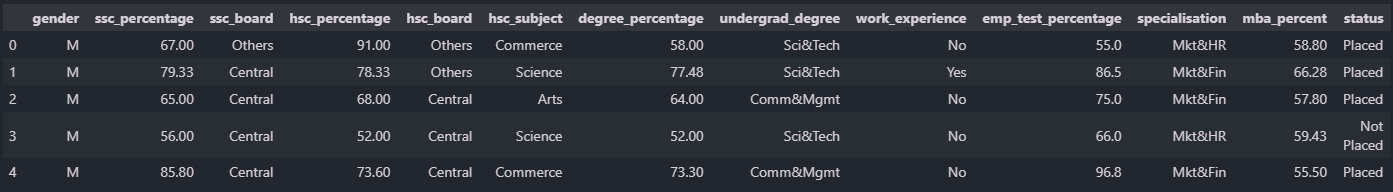
\includegraphics[scale=0.46]{csvimage.png}

    Table 2: Esempio dataset.csv
\end{center}

Si può vedere dalla \textit{Table 2} il dataset che abbiamo scelto per il nostro progetto.
Analizziamo l'influenza di ogni singola feature di questo dataset:

\begin{center}
    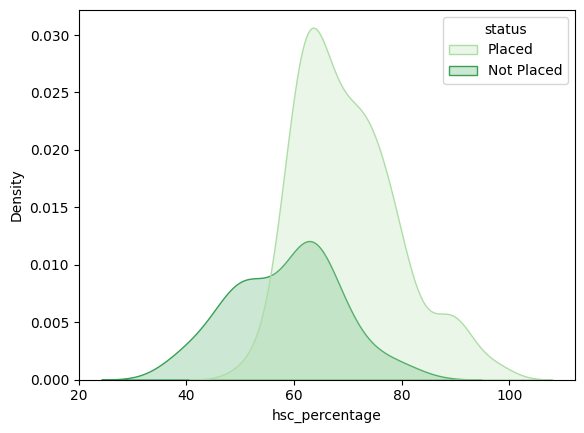
\includegraphics[scale=0.5]{hscpercentage.png}

    \textit{HSC Percentage}
\end{center}

Da questo grafico possiamo vedere che la variabile \textit{HSC Percentage} influisce nel dataset, perchè all'aumentare del valore (voto)
può incidere sulla previsione del modello.

Da questa considerazione abbiamo deciso di non eliminare questa variabile.

\begin{center}
    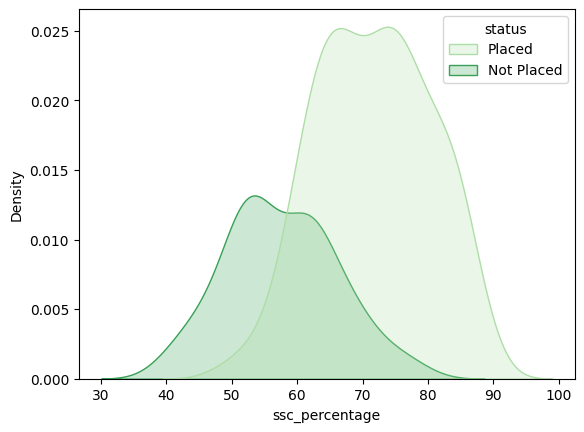
\includegraphics[scale=0.5]{sscpercentage.png}

    \textit{SSC Percentage}
\end{center}

Da questo grafico si può notare che la variabile \textit{SSC Percentage} influisce notevolmente nel dataset perchè come abbiamo visto con la
variabile \textit{HSC Percentage}, all'aumentare del valore aumenta anche la possibilità di essere piazzati.

Da questa considerazione abbiamo deciso di non eliminare questa variabile.

\begin{center}
    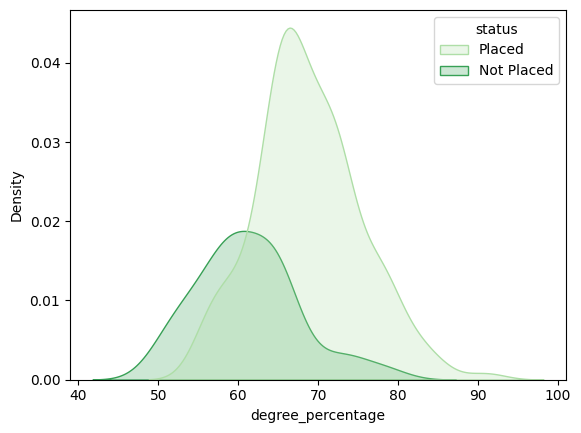
\includegraphics[scale=0.5]{degreepercentage.png}

    \textit{Degree Percentage}
\end{center}

Da questo grafico si può notare che la variabile \textit{Degree Percentage} influisce nel dataset, perchè all'aumentare del valore aumenta anche la possibilità
di essere piazzati.

Da questa considerazione abbiamo deciso di non rimuovere questa variabile.

\begin{center}
    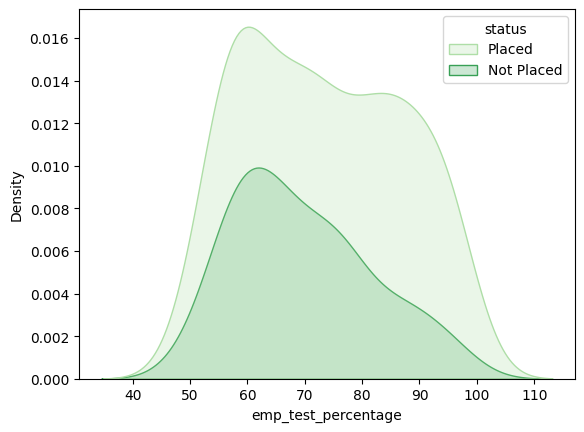
\includegraphics[scale=0.5]{emptestpercentage.png}

    \textit{EmpTest Percentage}
\end{center}

Come si nota da questo grafico la variabile \textit{EmpTest Percentage} influisce di poco nel dataset, perchè all'aumentare del valore aumenta leggermente la possibilità
di essere presi e non.

Da questa considerazione abbiamo deciso di rimuoverla.

\begin{center}
    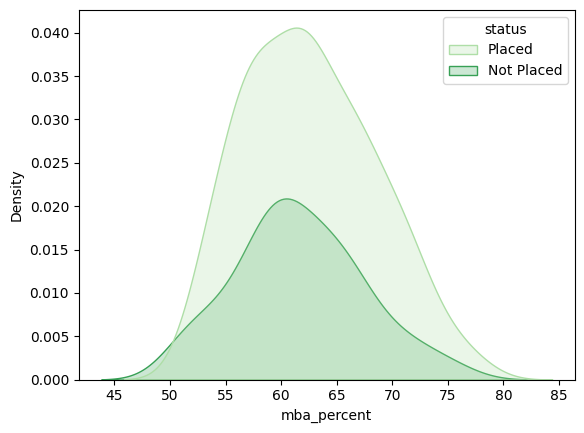
\includegraphics[scale=0.5]{mbapercentage.png}

    \textit{MBA Percentage}
\end{center}

Come si nota da questo grafico la variabile \textit{MBA Percentage} influisce di poco nel dataset, perchè all'aumentare del valore aumenta leggermente la possibilità di essere presi o non.

Da questa considerazione abbiamo deciso di rimuovere la variabile.

\begin{center}
    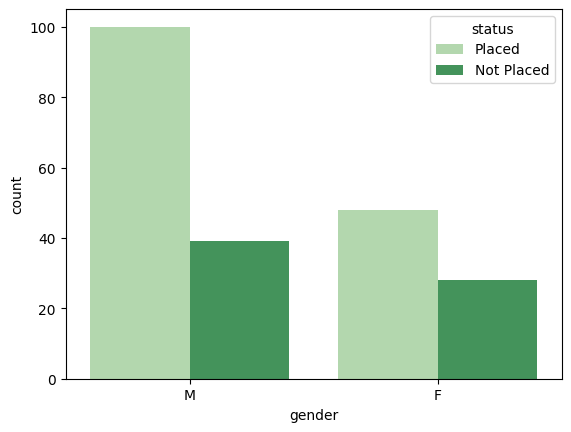
\includegraphics[scale=0.5]{gender.png}

    \textit{Gender}
\end{center}

Come è evidente dal grafico la variabile \textit{Gender} influisce notevolmente nel dataset, tanto che il numero di uomini piazzati è maggiore rispetto alle donne. Questo influenzerebbe il modello, portandolo anche a dare una previsione discriminatoria per un gender.
Alla luce di questo abbiamo deciso di rimuovere la variabile \textit{Gender} così da rendere il modello quanto più imparziare possibile da un punto di vista \textbf{Etico.}

\begin{center}

    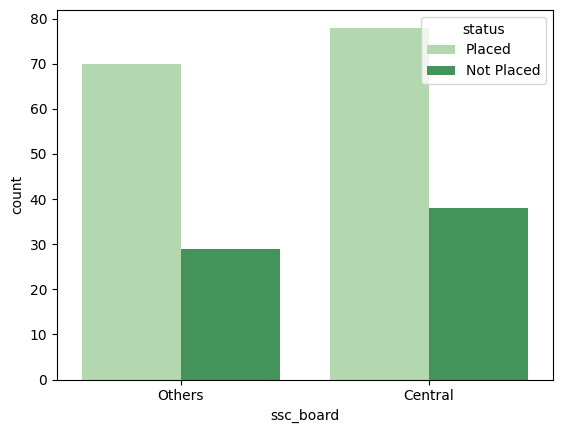
\includegraphics[scale=0.5]{sscboard.png}

    \textit{SSC Board}
\end{center}
Come si può vedere da grafico, la variabile \textit{SSC Board} influisce discretamente nel dataset, in quanto in base al valore della variabile, non c'è una differenza notevole tra le possibilità di essere preso o non. Quando la variabile ha come valore "Others", abbiamo una probabilità lievemente maggiore di essere piazzati rispetto al valore "Central".
Nonostante questo, abbiamo deciso di non rimuovere la variabile.

\begin{center}
    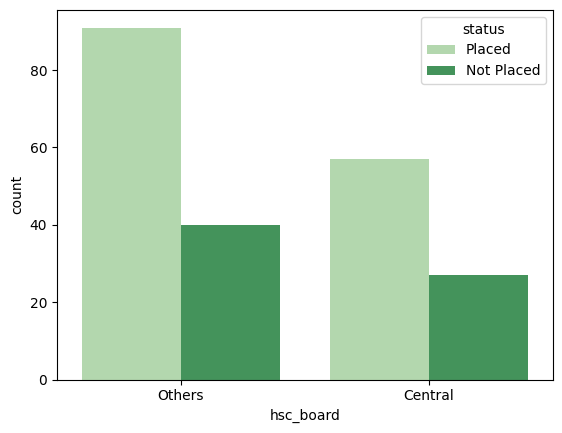
\includegraphics[scale=0.5]{hscboard.png}

    \textit{HSC Board}
\end{center}
Come si può notare dal grafico, la variabile \textit{HSC Board} influisce notevolmente nel dataset, in quanto in base al valore della variabile, la probabilità di essere piazzato è notevole.
In conclusione abbiamo deciso di non rimuovere la variabile.
\begin{center}
    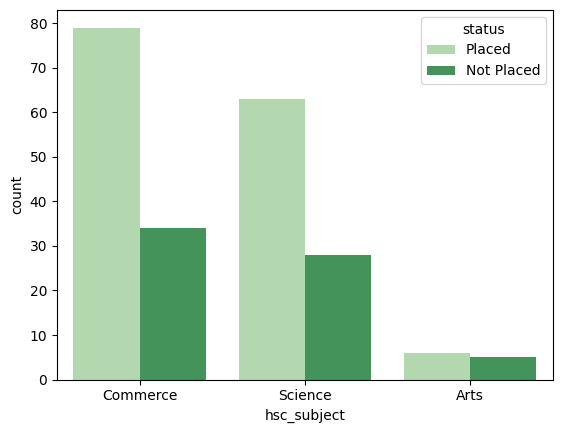
\includegraphics[scale=0.5]{hscsubject.png}

    \textit{HSC Subject}
\end{center}
Come si può vedere dal grafico di sopra, la variabile \textit{HSC Subject} influisce nel dataset, in quanto in base al valore della variabile, si potrebbe avere più possibilità di essere presi o non. In questo caso il valore "Commerce" aumenterebbe le possibilità di essere presi per una persona che ha studiato in questo campo.
Da questa considerazione abbiamo deciso di non rimuoverla.
\begin{center}
    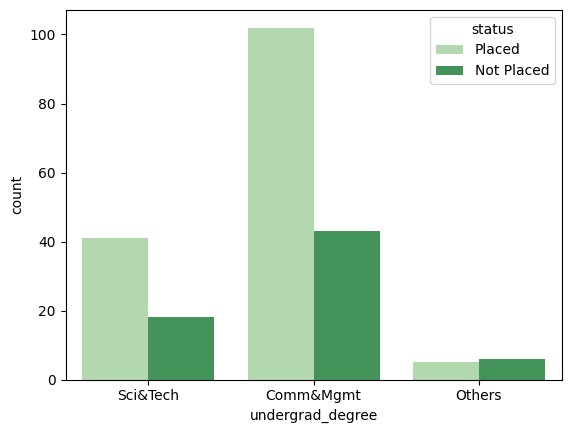
\includegraphics[scale=0.5]{undergraddegree.png}

    \textit{Undergrad Degree}
\end{center}
Come si può vedere dal grafico di sopra, la variabile \textit{Undergrad degree} influisce nel dataset, in quanto in base al valore della variabile, si avrà una probabilità maggiore di essere presi o non. Si può notare infatti che le persone che si sono laureate nel campo "Comm\&Mgmt" hanno più possibilità di essere presi.
Da questa analisi abbiamo deciso di non rimuovere la variabile.
\begin{center}
    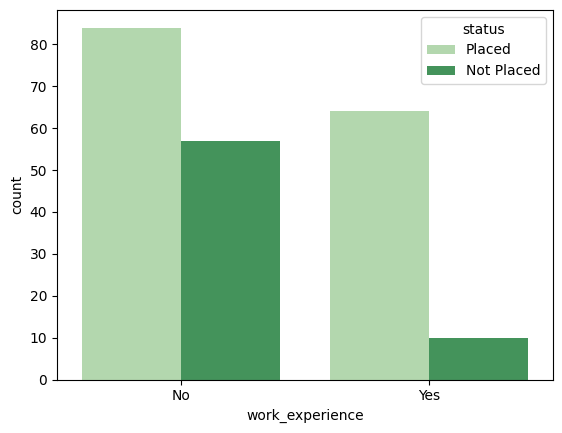
\includegraphics[scale=0.5]{workexperience.png}

    \textit{Work Experience}
\end{center}
Come si può vedere da questo grafico, la variabile \textit{Work experience} influisce nel dataset. Chi non ha esperienze lavorative, ha più possibilità di essere preso rispetto a chi ne ha.
In conclusione abbiamo deciso di non rimuoverla.
\begin{center}
    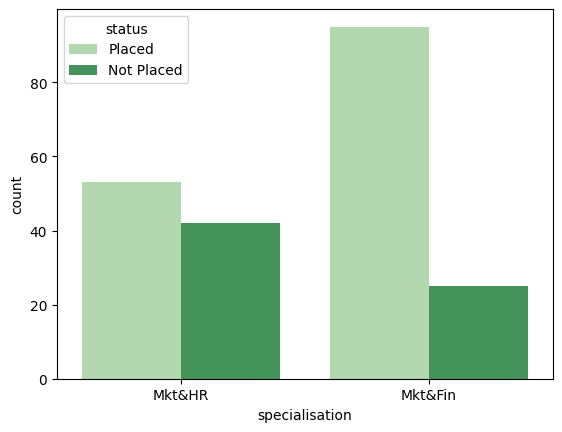
\includegraphics[scale=0.5]{specialisation.png}

    \textit{Specialisation}
\end{center}
In questo grafico la variabile \textit{Specialisation} influisce nel dataset. Chi ha un certo tipo di specializzazione, come "Mkt\&Fin", ha più possibilità di essere preso.
In conclusione abbiamo deciso di non rimuovere la variabile.

\subsubsection{Data balancing}
Il \textit{Data Balancing} è l'insieme di tecniche per convertire un dataset sbilanciato in un dataset bilanciato.
Questa è una delle fasi più importanti del \textbf{Data Preparation} perchè molti problemi reali sono sbilanciati e
la maggior parte dei Machine Learning funzionano bene solo quando il numero di esempi di una certa classe è simile al numero di esempi di un'altra classe.
\par
Questa per noi è una delle fasi più importanti per il nostro progetto avendo un numero di istanze di una classe estremamente diversa da un altra.
Analizziamo ora com'è bilanciato il nostro dataset:

\begin{center}
    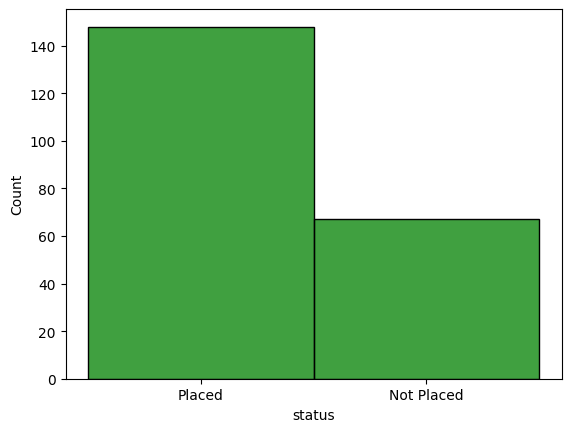
\includegraphics[scale=0.6]{istance_1.png}
\end{center}

Dal grafico si evince che non abbiamo un numero di istanze della classe \textit{Not Placed} uguale alla classe \textit{Placed}, oltretutto è un numero largamente inferiore (Placed: 148, Not Placed: 67).
\par
Dopo una serie di analisi siamo arrivati alla conclusione di utilizzare una tecnica di OverSampling, che sarebbe un metodo in cui vengono casualmente aggiunte un numero di istanze del dataset della classe di minoranza, che in questo caso è \textit{Not Placed}.
\par
Utilizzando la classe RandomOverSampler siamo riusciti a bilanciare il nostro dataset.
\par
Di seguito viene mostrato il grafico una volta svolta questa operazione:

\begin{center}
    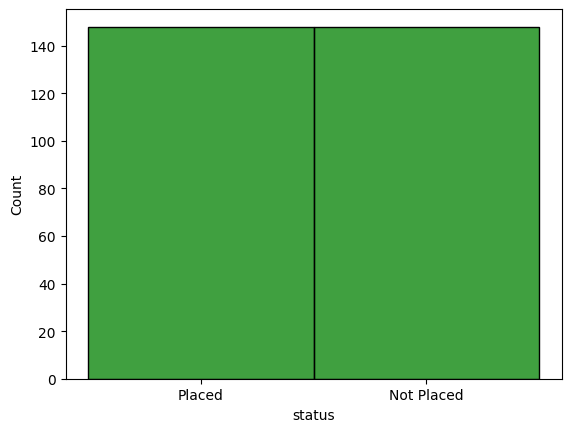
\includegraphics[scale=0.6]{istance_2.png}
\end{center}

Tutto questo ci ha permesso quindi di migliorare le performance del nostro modello di Machine Learning, portandoci alla conclusione del nostro \textbf{Data Preparation}. Da adesso andremo a esporre il nostro modello di
Machine Learning.

\subsection{Modelling}
In questa fase valuteremo la tecnica di Machine Learning da utilizzare.

Come abbiamo definito in precedenza utilizzeremo un modello di \textit{Machine Learning} supervisionato che andrà a risolvere problemi
di classificazione.

\subsubsection{Classificazione}
La classificazione è una task in cui l'obbiettivo è predire il valore di una variabile categorica, chiamata variabile
dipendente tramite l'utilizzo di un training set, ovvero un insieme di osservazioni per cui la variabile dipendente è nota.
\par
Esistono dei problemi di classificazione che possono essere risolti tramite l'utilizzo di un modello chiamato classificatore. Nel nostro caso abbiamo analizzato diversi modelli:

\begin{itemize}
    \item \textbf{Decision Tree}.
    \item \textbf{Random Forest}.
    \item \textbf{Naive Bayes}.
    \item \textbf{K-Nearest Neighbors}.
\end{itemize}
Ogni classificatore è stato analizzato attraverso l'uso di metriche di valutazione che sono servite anche per aiutarci sulla scelta del Modello da utilizzare.
Di seguito spiegheremo ogni modello e il suo obiettivo.

\subsubsection{Decision Tree}
Il Decision Tree (Albero Decisionale) è un modello di Machine Learning può essere utilizzato anche per problemi di  classificazione. In questo modello, l'algoritmo cosrtuisce un albero di decisione che rappresenta
la sequenza di decisioni che devono essere prese per classificare correttamente un'istanza. L'obiettivo di questo algoritmo è quello di predire il valore di una variabile target, apprendendo semplici regole di decisione inferite dai dati di training.
La particolarità di questi alberi è la loro facilità di lettura, grazie al quale è possibile comprendere la ragione con la quale è stata fatta una determinata predizione.

\subsubsection{Random Forest}
Il Random Forest è un modello di Machine Learning utilizzato per la classificazione e va a combinare molteplici alberi decisionali in un unico modello. In poche parole vengono costruiti questi alberi
decisionali utilizzando sottoinsiemi casuali del set di dati di training e selezionando casualmente le variabili da utilizzare in ciascun albero.

\subsubsection{Naive Bayes}
Il Naive Bayes è un modello di Machine Learning utilizzato per la classificazione che va a considerare le caratteristiche della nuova istanza da classificare e calcola la probabilità che queste facciano parte di una classe
tramite l'applicazione del teorema di Bayes.

\subsubsection{K-Nearest Neighbors}
Il K-Nearest Neighbors è un modello di Machine Learning utilizzato per la classificazione che va a rappresentare delle istanze di training come punti nello spazio multidimensionale, dove ogni dimensione
rappresenta una variabile del problema.

\subsubsection{Training set e Test set}
Come si è potuto notare dai paragrafi precedenti, la preparazione dei dati è molto importante perché poi quest'ultimi dovranno essere utilizzati della fase di addestramento per il nostro modello. Una cosa importante che bisogna ricordarsi è che non si deve far allenare il Machine Leaner con
l'intero dataset perché può portare a risultati totalmente inaffidabili. Per questo motivo bisogna dividere il dataset  in due insiemi: Training set e Test set. Il Training set è un insieme di dati che il nostro algoritmo utilizzerà per l'addestramento, mentre il Test Set verrà utilizzato dall'algoritmo
addestrato per mettersi alla prova perché dovrù predire la classe di appartenenza di questi dati.
Per il nostro modello abbiamo deciso di dividere il dataset in un buon 67\% per il Training set e il restante 33\% per il Test set.

\subsubsection{Validation}
Da questo momento inizieremo a valutare i modelli precedentemente descritti per decidere quale utilizzare nel nostro progetto.
Ovviamente avremo bisogno di qualche metrica da utilizzare per verificare le prestazioni del nostro modello nella fase di training. Di sotto sono elencate le metriche che andremo a utilizzare e valutare per ogni singolo modello:
\begin{itemize}
    \item \textbf{Acuratezza}: indica il numero totale di predizioni corrette, sia della classe positiva che negativa.\par \[\textit{Accuracy}=\frac{(TP + TN)}{(TP+TN+FP+FN)} \]
    \item \textbf{Precisione}: indica il numero di predizioni corrette delle classe \textbf{True} rispetto tutte le predizioni fatte dal classificatore. In poche parole indica quanti errori ci saranno nella lista delle predizioni fatte dal classificatore.\par \[\textit{Precision}=\frac{(TP)}{(TP+FP)} \]
    \item \textbf{Recall}: indica il numero di predizioni corrette per la classe \textbf{True} rispetto tutte le istanze positive di quella classe. In breve indica quante istanze positive nell'intero dataset il classificatore può determinare.\par \[\textit{Recall}=\frac{(TP)}{(TP+FN)} \]
\end{itemize}
Vogliamo massimizzare ognuno di questi valori nella loro interezza.
Elenchiamo adesso i vari modelli con i relativi valori delle metriche:
\begin{itemize}
    \item \textbf{Decision Tree}
          \begin{itemize}
              \item \textbf{acuratezza}: 0.85
              \item \textbf{precisione}: Placed: 0.85, Not Placed: 0.84
              \item \textbf{recall}: Placed: 0.80, Not Placed: 0.89
          \end{itemize}
    \item \textbf{Random Forest}
          \begin{itemize}
              \item \textbf{acuratezza}: 0.87
              \item \textbf{precisione}: Placed: 0.84, Not Placed: 0.89
              \item \textbf{recall}: Placed: 0.86, Not Placed: 0.87
          \end{itemize}
    \item \textbf{Naive Bayes}
          \begin{itemize}
              \item \textbf{acuratezza}: 0.68
              \item \textbf{precisione}: Placed: 0.64, Not Placed: 0.72
              \item \textbf{recall}: Placed: 0.66, Not Placed: 0.70
          \end{itemize}
    \item \textbf{K-Nearest Neighbors}
          \begin{itemize}
              \item \textbf{acuratezza}: 0.82
              \item \textbf{precisione}: Placed: 0.76, Not Placed: 0.88
              \item \textbf{recall}: Placed: 0.78, Not Placed: 0.86
          \end{itemize}
\end{itemize}
Da questa analisi possiamo vedere che i modelli Decision Tree e Random Forest sono tra quelli più promettenti, con delle metriche abbastanza alte.
La decisione del modello alla fine è ricaduta nel Random Forest, in quanto offriva dei valori piuttosto bilanciati e migliori rispetto al Decision Tree.
\subsection{Evaluation}
Questa è la fase in cui valuteremo i nostri risultati finali perché poi dovremo passare alla fase di \textbf{Deployment}. Da qui capiremo se i nostri obiettivi di business sono stati rispettati, se le nostre analisi sono state corrette e se il nostro progetto è consistente e solido.
Durante il nostro lavoro, abbiamo sempre avuto dubbi riguardo il raggiungimento del nostro obiettivo, siamo dovuti ritornare indietro nei nostri passi in certi casi per errori in fase di analisi o perché ci sono stati problemi in fase di modelling.
Precedentemente avevamo pensato di renderlo utilizzabile per studenti italiani, però quando abbiamo verificato che ciò non poteva realizzarsi per il dataset che avevamo deciso di utilizzare, siamo ritornati indietro rianalizzando i dati offerti e rifacendo la fase di \textbf{Data Preparation}.
Oltrettutto la nostra preoccupazione era dovuta alla scelta di lasciare o meno una determinata feature \textbf{(Gender)}, che per noi era trascurabile però influenzava notevolmente la predizione del nostro Modello. Alla fine i risultati usciti sono soddisfacenti, coerenti e quanto più solidi possibili tanto da rendere possibile la fase di \textbf{Deployment}.
\subsection{Deployment}
In questa fase parleremo di come abbiamo implementato il nostro modello di \textbf{Intelligenza Artificiale}.
\par
Come precedentemente avevamo descritto nella fase di \textit{Business Understanding}, abbiamo utilizzato \textbf{Python} come linguaggio di programmazione del nostro modello che offriva una serie di librerie interessanti e utili come \textit{Pandas, Sklearn, Seaborn, RandomOverSampler, CustomTkinter} e altri moduli utili per i modelli che abbiamo testato.
\par
Per esempio abbiamo importato all'interno del nostro codice il modulo \textit{RandomForestClassifier}, che appunto sfruttava l'algoritmo Random Forest.
Com'è possibile vedere dalla nostra pagina \textbf{GitHub} \textit{(ref. parag. 1.1 pg. 3)}, è stato  suddiviso il nostro programma in directory dov'è possibile vedere il codice sorgente suddiviso in due parti:
\begin{enumerate}
    \item \textbf{Business Logic}, che presenta la parte logica dell'applicativo e che integra il modello di Machine Learning.
    \item \textbf{View}, che presenta la GUI del tool.
\end{enumerate}
Alla fine siamo riusciti a integrare il modello di Machine Learning nel modo più completo possibile e terminare il nostro Tool.

\section{Conclusione}
Il progetto si può dire concluso, dopo il tanto lavoro e impegno nella fase di modellazione del tool e del modello presentato.
Un grande scalino, come descritto nella fase di \textit{Data Understanding} e un pò in tutto il documento è stato il discorso dell'\textbf{Etica},
il tutto anche dovuto alla difficoltà nella fase di ricerca del/dei dataset, in questo questo caso unico, in quanto molti dataset non tornavano utili per il nostro
progetto. Con questo però non si pregiudica in futuro la possibilità di aggiungere altri dati e rendere il modello ancora più efficace e veritiero possibile e che sia
in futuro utilizzabile da più studenti di Nazioni diverse.
\par
In questa conclusione vogliamo ovviamente dire di essere enormemente soddisfatti del progetto che è stato creato e concluso, soprattutto per il nostro primo progetto che integra un modello di \textbf{Intelligenza Artificiale.}

\end{document}
